\chapter[The 25$^{\text{th}}$ of January 2024 - First results \& comments about HiDeNN]{First results \& comments about HiDeNN}

\begin{chapabstract}
    This chapter gives first results and comments about HiDeNNs
\end{chapabstract}

\minitoc

\section{Loss function}
Just like with regular PINNs, the loss function constrains the neural network to be physically consistent.
\subsection{Physical term}
 The first possibility is to use the potential energy of the system 
\begin{equation}
    \mathcal{L} = J\left(\vect{u}\right) = \frac{1}{2}\int_{\Omega} AE\left(\frac{\mathrm{d}\vect{u}}{\mathrm{d}x}\right)^2\mathrm{d}x - \int_{\Omega} \vect{u} \cdot \vect{b} \mathrm{d}x
\end{equation}
as a loss function as the solution minimises the potential energy. A disadvantage of doing so is that there are no easily chosen criteria to stop the training as the loss function drops below zero without any prior knowledge of the inferior bound of such a function as shown in \cref{fig:Loss_zoom}.

\begin{figure}
    \centering
    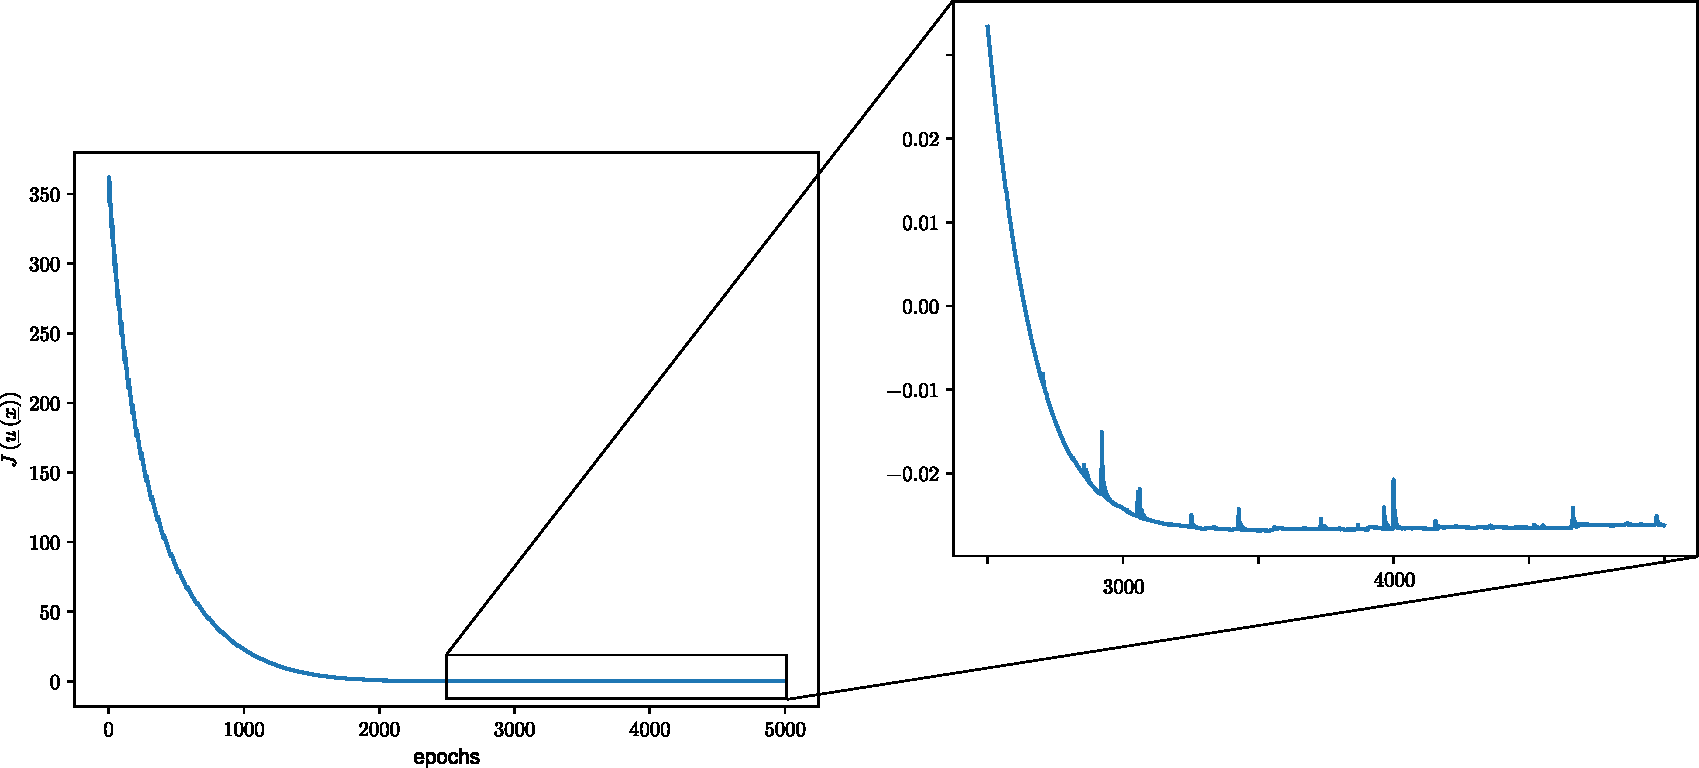
\includegraphics[width=\linewidth]{Figures/Loss_with_zoom.pdf}
    \caption{Potential energy $J\left(\vect{u}\right)$}
    \label{fig:Loss_zoom}
\end{figure}

A comparison of the information given by the decrease of the loss and the decrease of the $\ell^2$-error is given in \cref{fig:L2_vs_PE}, which highlights that the global behaviour of decay of both indicators agrees reasonably well.

\begin{figure}
    \centering
    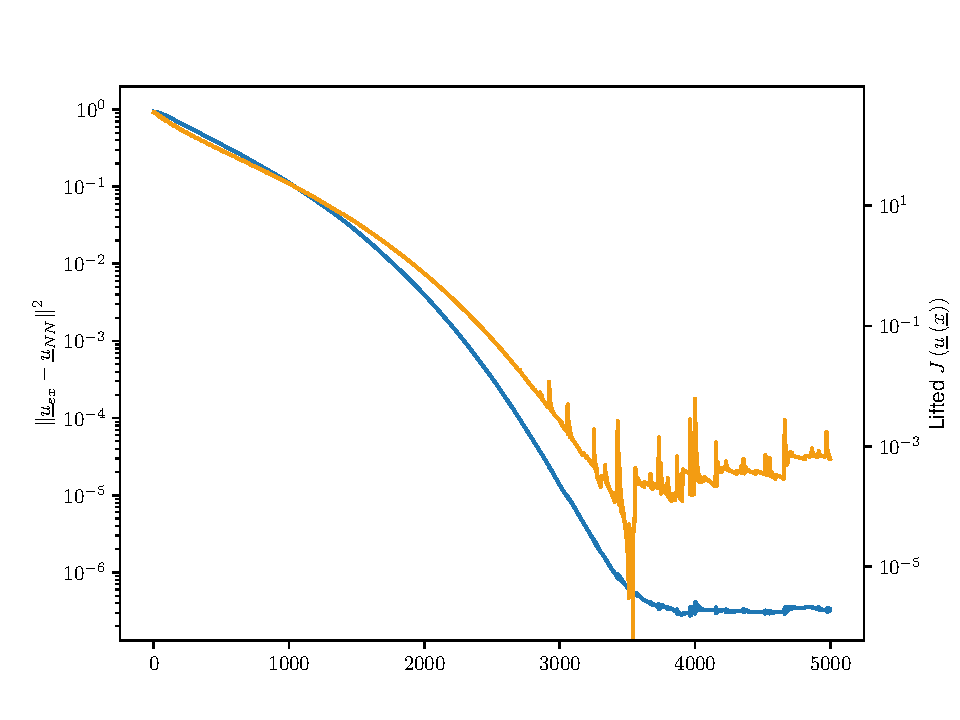
\includegraphics[width=0.7\linewidth]{Figures/Loss_Comaprison.pdf}
    \caption{Lifted $\mathcal{L}$ compared to  $\ell^2$-error}
    \label{fig:L2_vs_PE}
\end{figure}

\subsection{Regularisation term}

In order to avoid having distorted or even inside-out elements, a regularisation term is proposed so that the loss reads

\begin{equation}
    \mathcal{L} \triangleq\underbrace{ \mathcal{J\left(\vect{u}\right)} }_{\text{Physical loss}} + ~\alpha \underbrace{\left(\frac{\max J\left(x_i\right)}{\min J\left(x_i\right)} - 1\right)}_{\text{Mesh regularisation}},
\end{equation}
where 
\begin{equation}
    \left(\frac{\max J\left(x_i\right)}{\min J\left(x_i\right)} - 1\right) \ge 0
\end{equation}
and $\alpha$ is a weight for the regularisation term.

\Rqs{This implies using additional hyper-parameters whose choice needs to be automated}{This tends to force the mesh to be uniform, so it might not be optimal in the future when we want localised refinements.}
\section{First results with $n_p=23$ \& $n_p=10$}
\subsection{Without regularisation}
The HiDeNN set up with the ADAM optimiser and allowing both the nodes coordinates and nodal values to be trained leads to the following results given in \cref{fig:FirstSol}. Here no regularisation is used, the nodes are just forbidden to cross one another.
\begin{figure}
    \begin{subfigure}{0.5\linewidth}
        \centering
        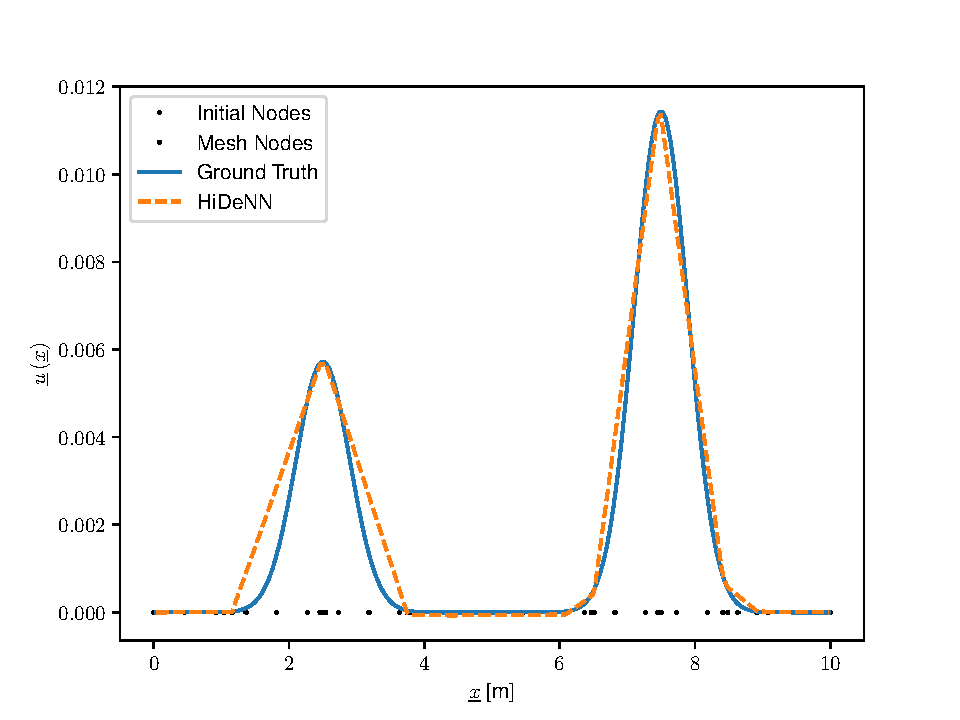
\includegraphics[width=\linewidth]{Figures/Solution_displacement.pdf}
        \caption{Displacement solution}
    \end{subfigure}
    \begin{subfigure}{0.5\linewidth}
        \centering
        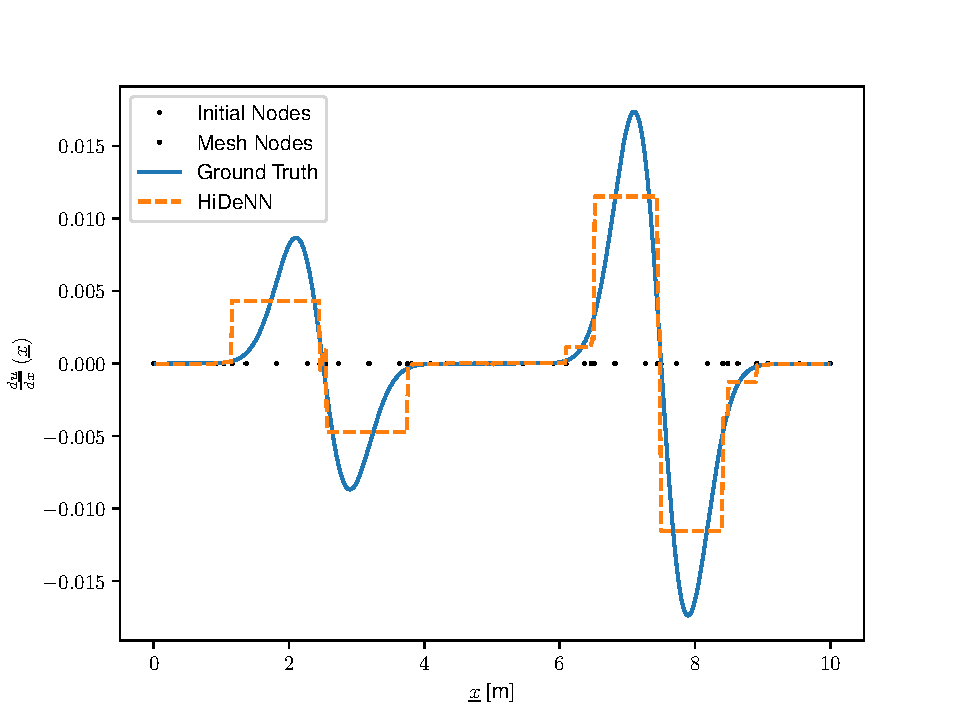
\includegraphics[width=\linewidth]{Figures/Solution_gradients.pdf}
        \caption{Displacement's first derivative}
    \end{subfigure}
    \caption{Comparison of NN's solutions with analytical solutions}
    \label{fig:FirstSol}
\end{figure}
The coordinates' optimisation process during training can be monitored by looking at their trajectories as shown in \cref{fig:Traj}.
\begin{figure}
    \centering
    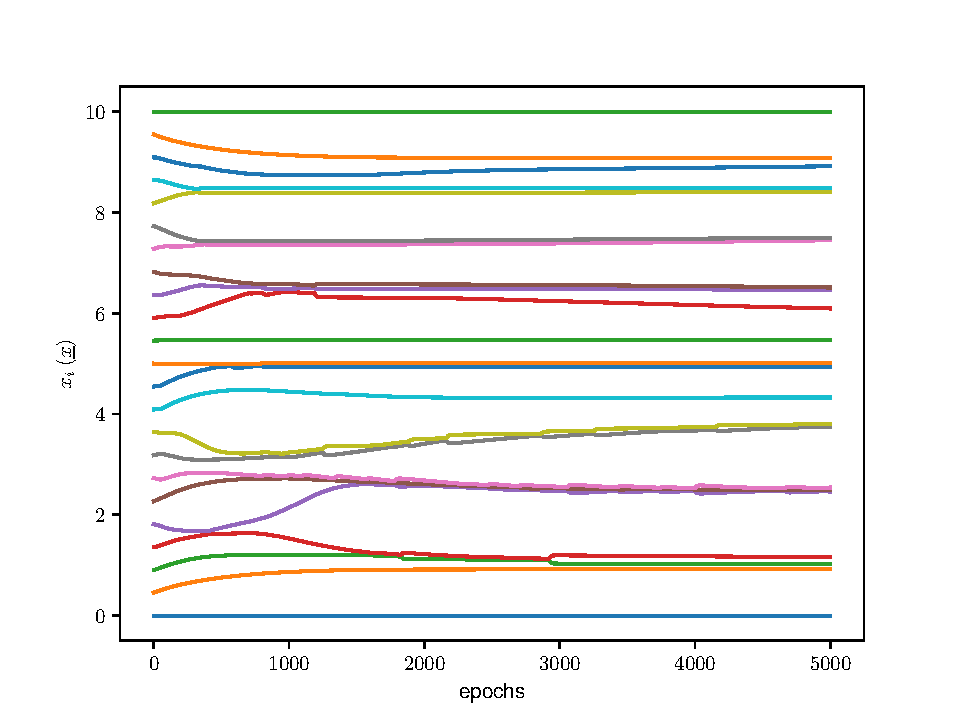
\includegraphics[width=0.5\linewidth]{Figures/Trajectories.pdf}
    \caption{Trajectories of the nodal coordinates without regularisation}
    \label{fig:Traj}
\end{figure}

\Rq{The nodes seem to be competing for the same position.}


\subsection{With regularisation (\& in double precision [\code{float64}])}

The comparison of the solution with the analytical solution is given in \cref{fig:FirstSol_regul}, and the loss and trajectories are given in \cref{fig:Loss_traj_regul}.
\begin{figure}
    \begin{subfigure}{0.5\linewidth}
        \centering
        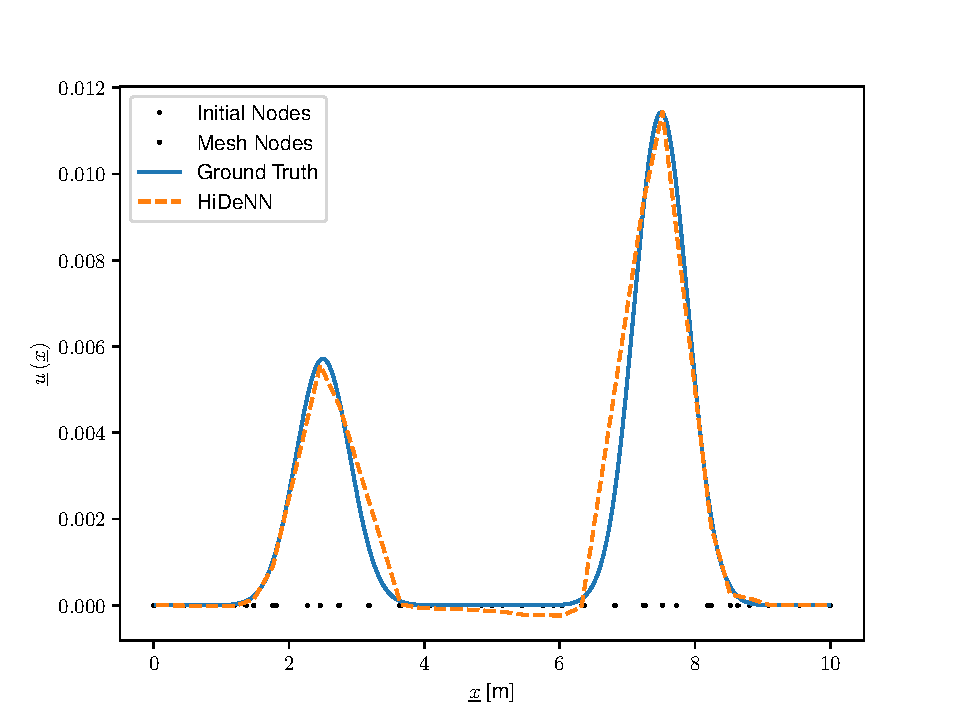
\includegraphics[width=\linewidth]{Figures/Solution_displacement_Regul64.pdf}
        \caption{Displacement solution}
    \end{subfigure}
    \begin{subfigure}{0.5\linewidth}
        \centering
        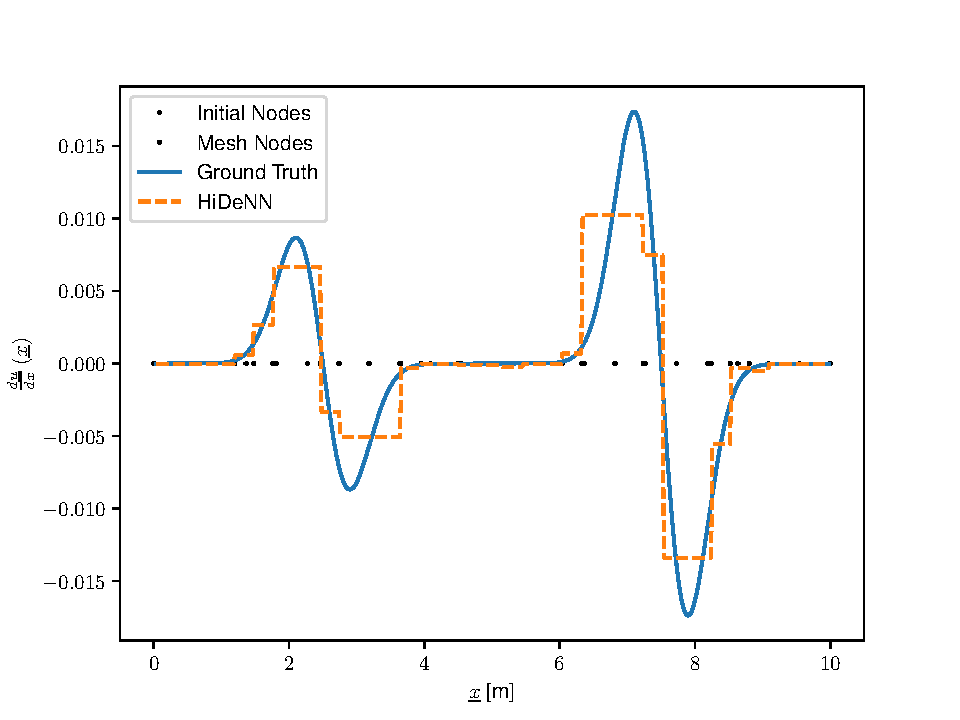
\includegraphics[width=\linewidth]{Figures/Solution_gradients_Regul64.pdf}
        \caption{Displacement's first derivative}
    \end{subfigure}
    \caption{Comparison of regularised NN's solutions with analytical solutions}
    \label{fig:FirstSol_regul}
\end{figure}
\begin{figure}
    \begin{subfigure}{0.5\linewidth}
        \centering
        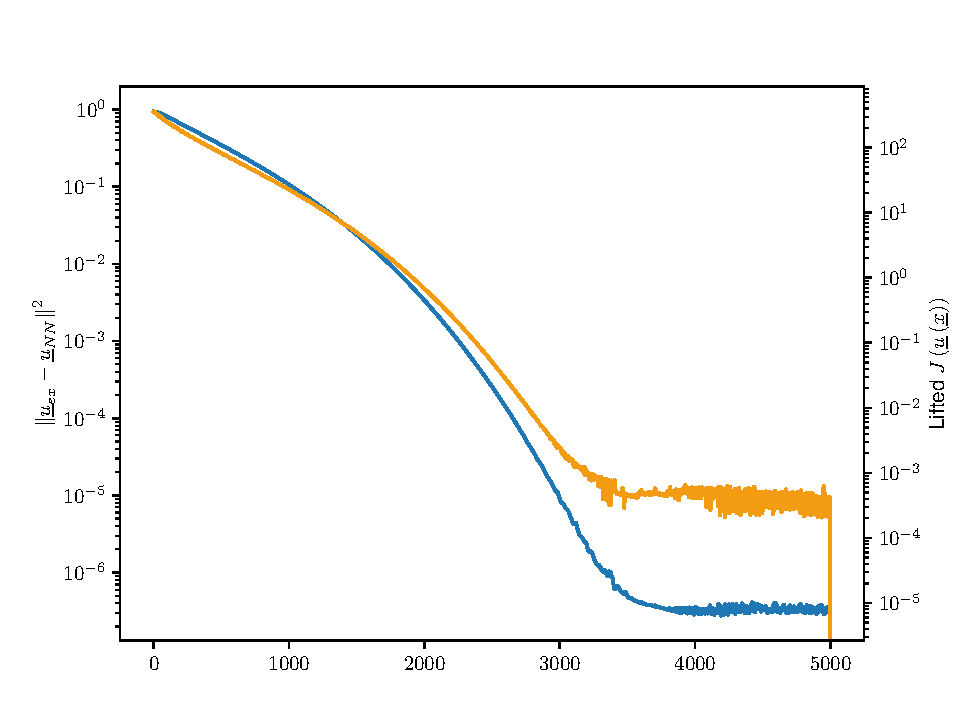
\includegraphics[width=\linewidth]{Figures/Loss_Comaprison_Regul64.pdf}
        \caption{Loss and $\ell^2$-error}
    \end{subfigure}
    \begin{subfigure}{0.5\linewidth}
        \centering
        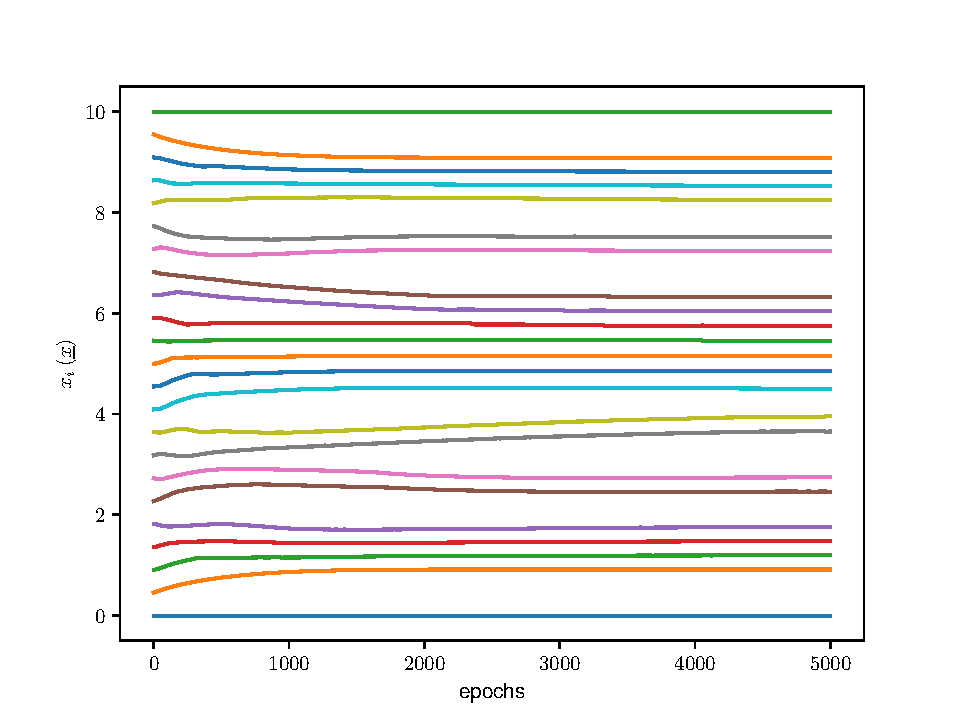
\includegraphics[width=\linewidth]{Figures/Trajectories_Regul64.pdf}
        \caption{Trajectories of the coordinates}
    \end{subfigure}
    \caption{Evolution of the loss and the $\ell^2$-error and evolution of the nodal coordinates with regularisation}
    \label{fig:Loss_traj_regul}
\end{figure}

\subsection{Influence of the mesh adaptivity}
\paragraph{$n_p=23$}
For $n_p=23$ the mesh adaptivity does not improve the solution

\begin{figure}
    \begin{subfigure}{0.3\linewidth}
        \centering
        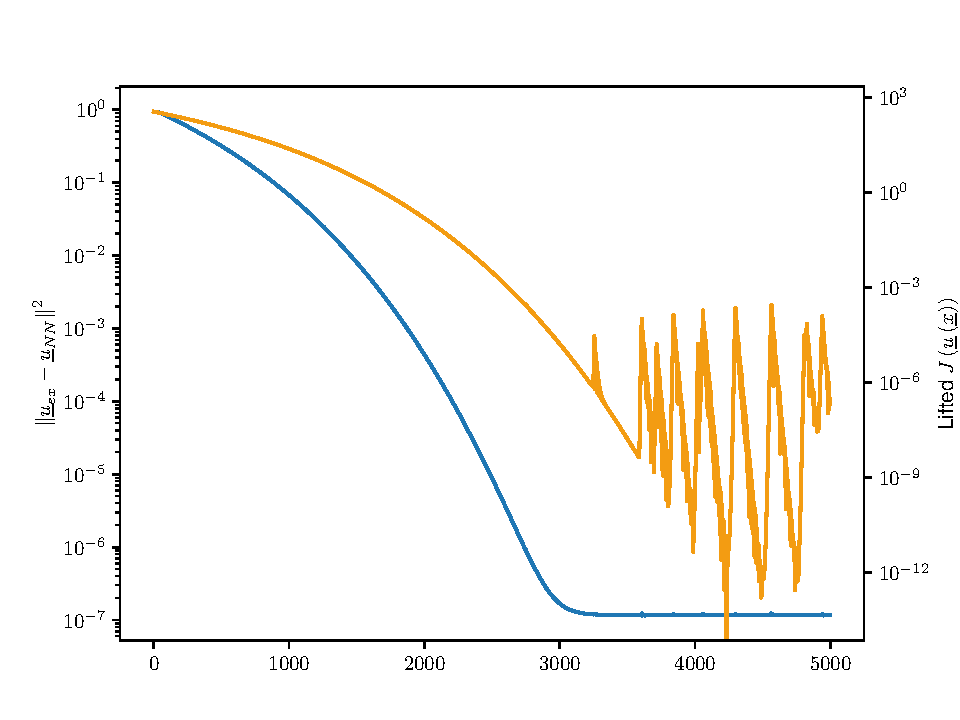
\includegraphics[width=\linewidth]{Figures/Loss_Comaprison_Frozen.pdf}
        \caption{Evolution of the loss}
    \end{subfigure}
    \begin{subfigure}{0.3\linewidth}
        \centering
        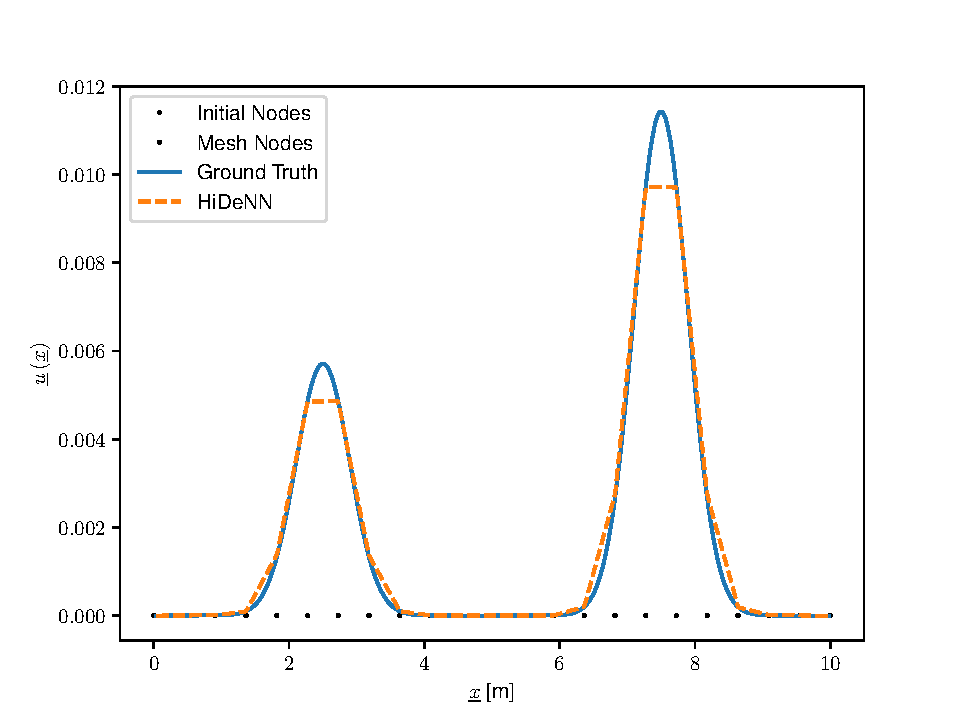
\includegraphics[width=\linewidth]{Figures/Solution_displacement_Frozen.pdf}
        \caption{Displacement}
    \end{subfigure}
    \begin{subfigure}{0.3\linewidth}
        \centering
        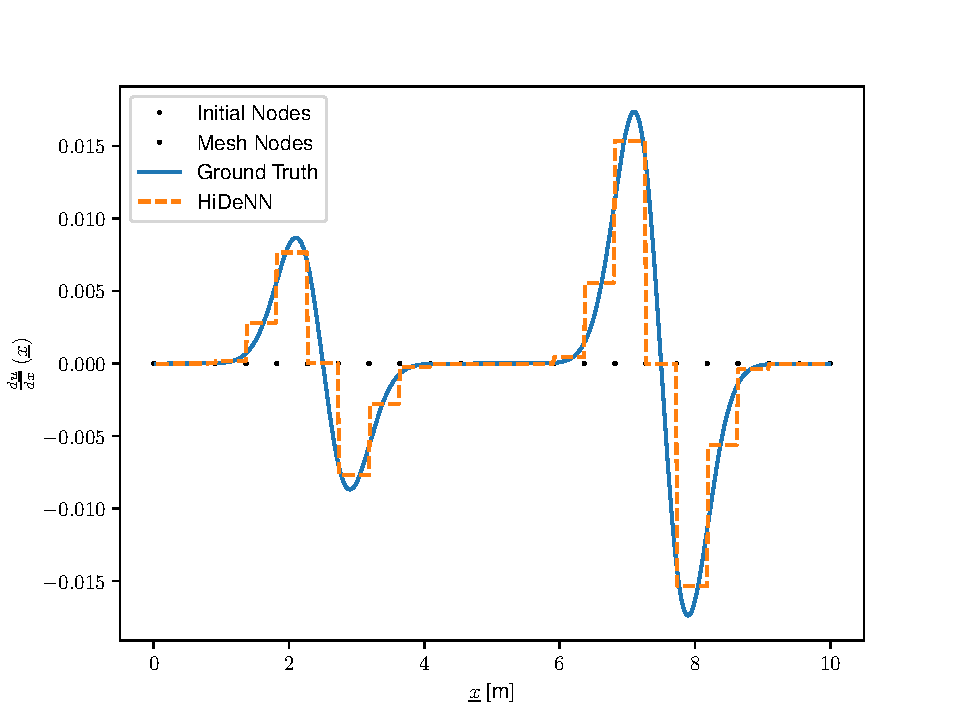
\includegraphics[width=\linewidth]{Figures/Solution_gradients_Frozen.pdf}
        \caption{Gradient}
    \end{subfigure}
    \caption{Fixed mesh - $n_p=23$}
    \label{fig:Fixed Mesh23}
\end{figure}

\begin{figure}
    \begin{subfigure}{0.3\linewidth}
        \centering
        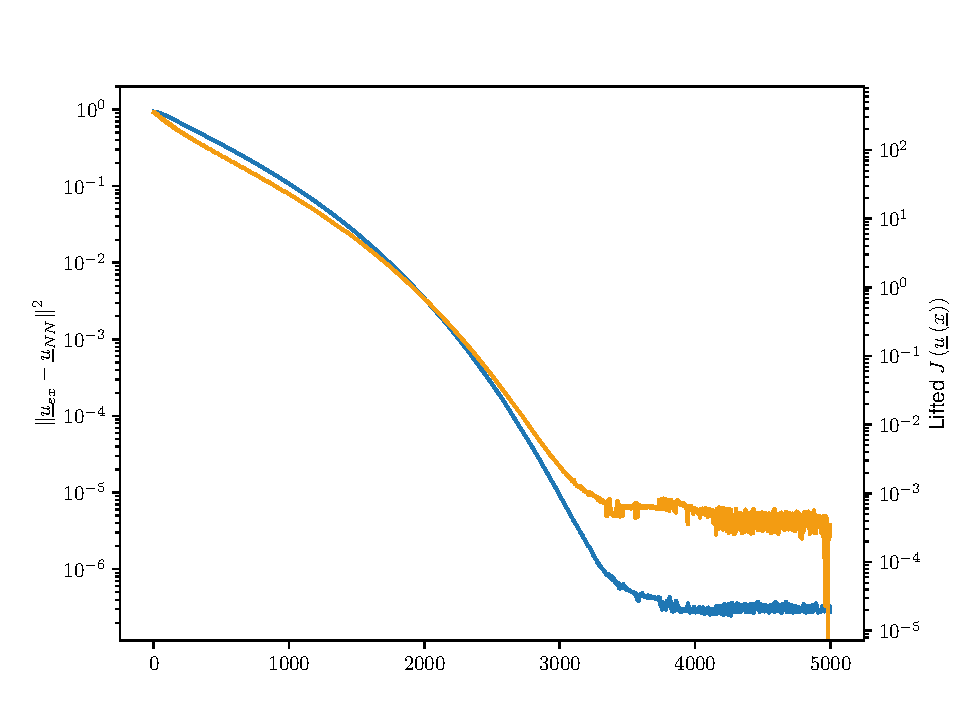
\includegraphics[width=\linewidth]{Figures/Loss_Comaprison_Regul32.pdf}
        \caption{Evolution of the loss}
    \end{subfigure}
    \begin{subfigure}{0.3\linewidth}
        \centering
        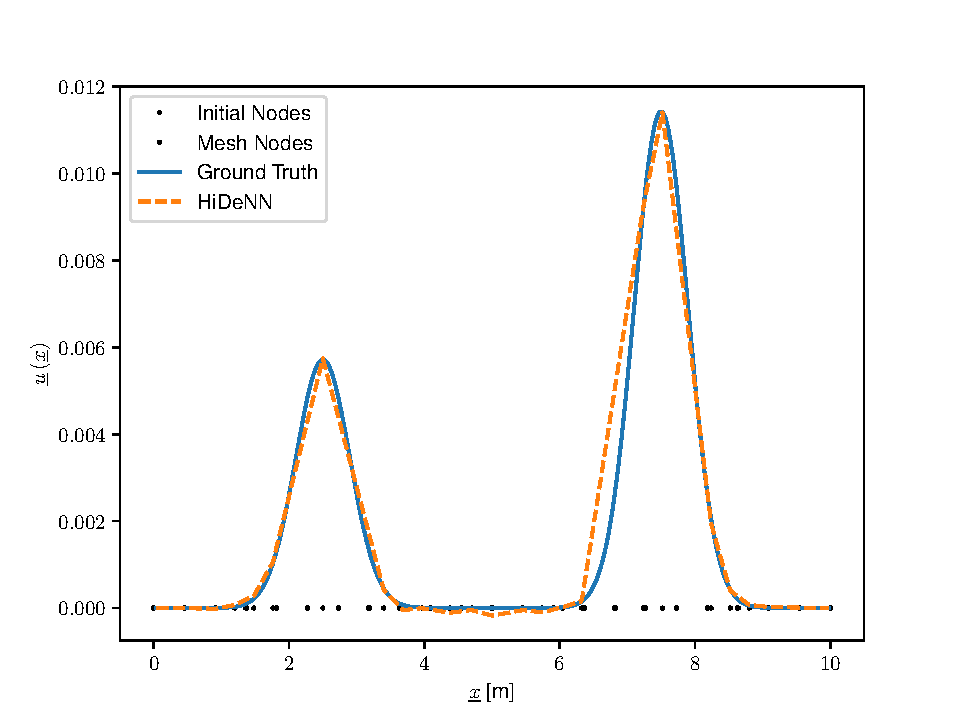
\includegraphics[width=\linewidth]{Figures/Solution_displacement_Regul32.pdf}
        \caption{Displacement}
    \end{subfigure}
    \begin{subfigure}{0.3\linewidth}
        \centering
        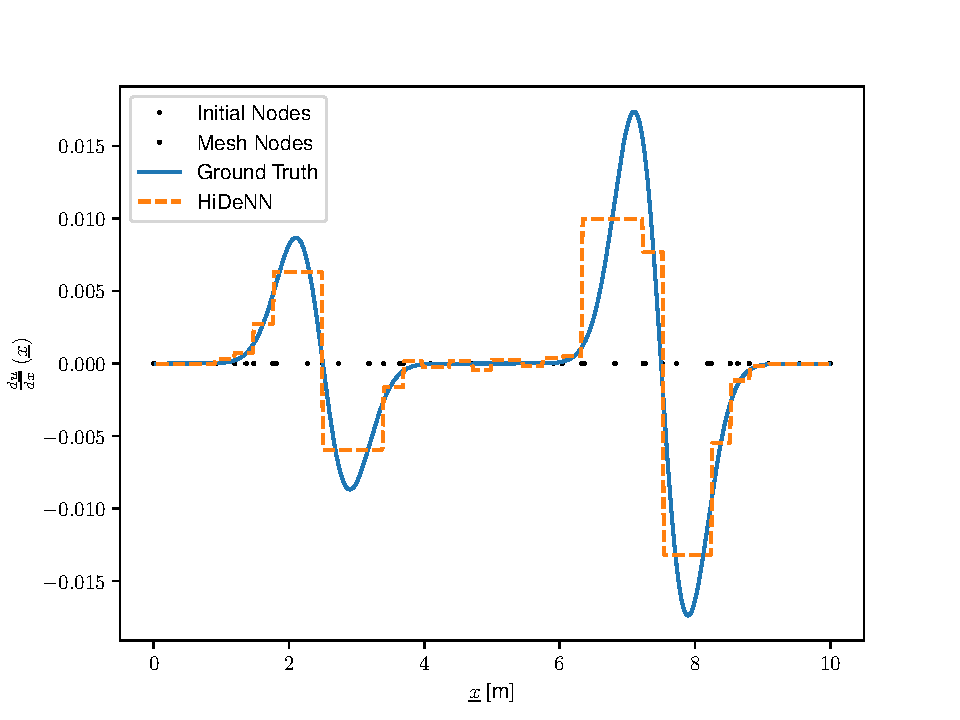
\includegraphics[width=\linewidth]{Figures/Solution_gradients_Regul32.pdf}
        \caption{Gradient}
    \end{subfigure}
    \caption{Free mesh float 32 - $n_p=23$}
    \label{fig:Fixed_Mesh23Float32}
\end{figure}

\begin{figure}
    \begin{subfigure}{0.3\linewidth}
        \centering
        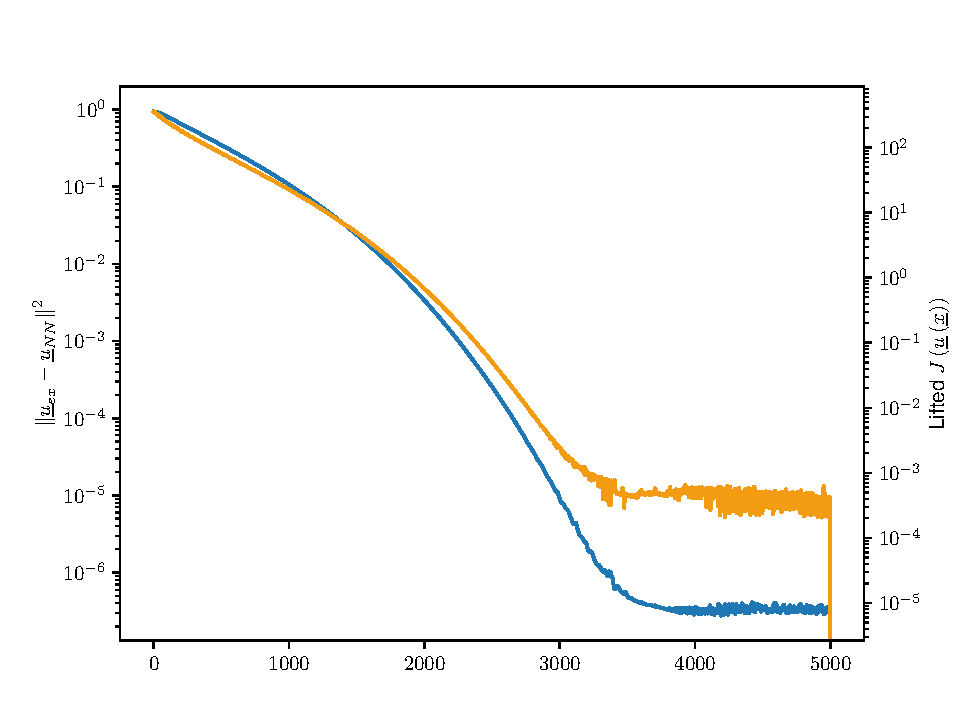
\includegraphics[width=\linewidth]{Figures/Loss_Comaprison_Regul64.pdf}
        \caption{Evolution of the loss}
    \end{subfigure}
    \begin{subfigure}{0.3\linewidth}
        \centering
        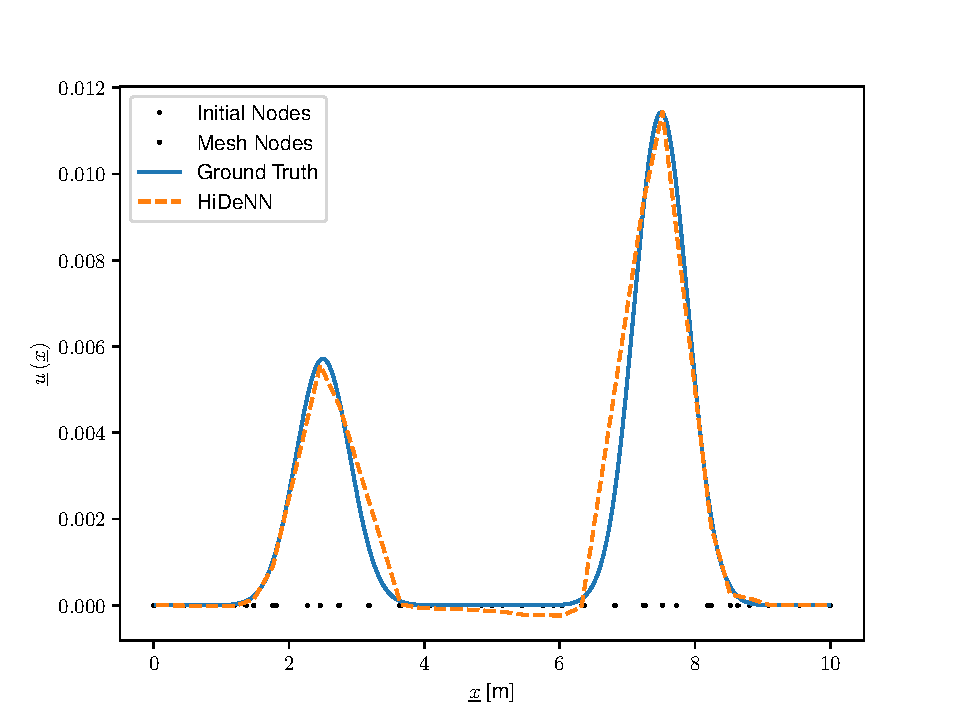
\includegraphics[width=\linewidth]{Figures/Solution_displacement_Regul64.pdf}
        \caption{Displacement}
    \end{subfigure}
    \begin{subfigure}{0.3\linewidth}
        \centering
        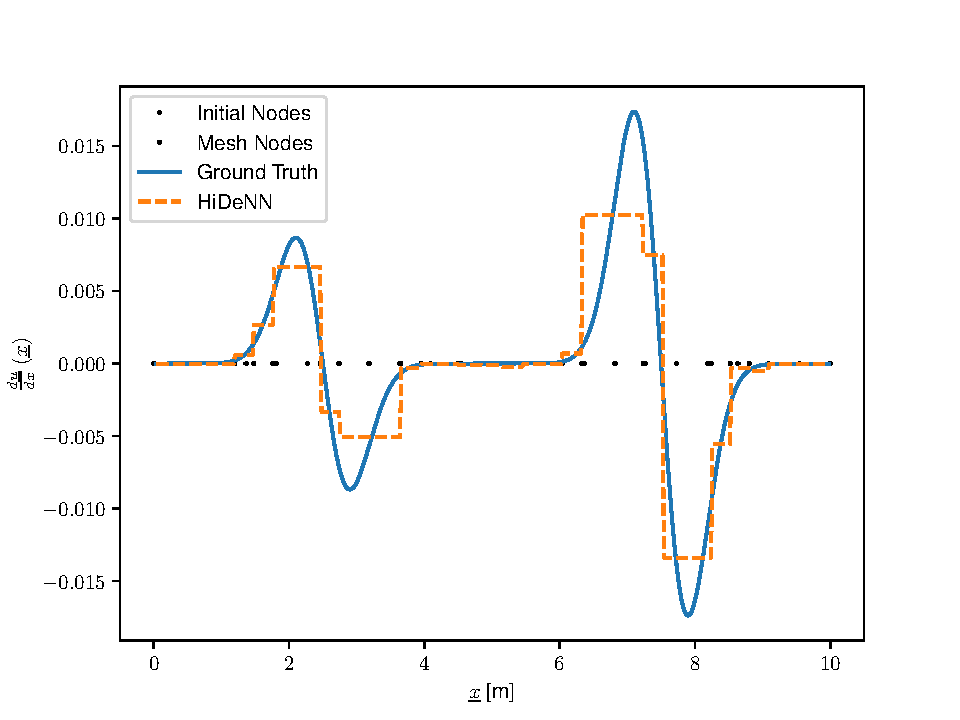
\includegraphics[width=\linewidth]{Figures/Solution_gradients_Regul64.pdf}
        \caption{Gradient}
    \end{subfigure}
    \caption{Free mesh float 64 - $n_p=23$}
    \label{fig:Fixed_Mesh23Float64}
\end{figure}


\paragraph{$n_p=10$}

For $n_p=10$ the mesh adaptivity improves the solution.


\begin{figure}
    \begin{subfigure}{0.3\linewidth}
        \centering
        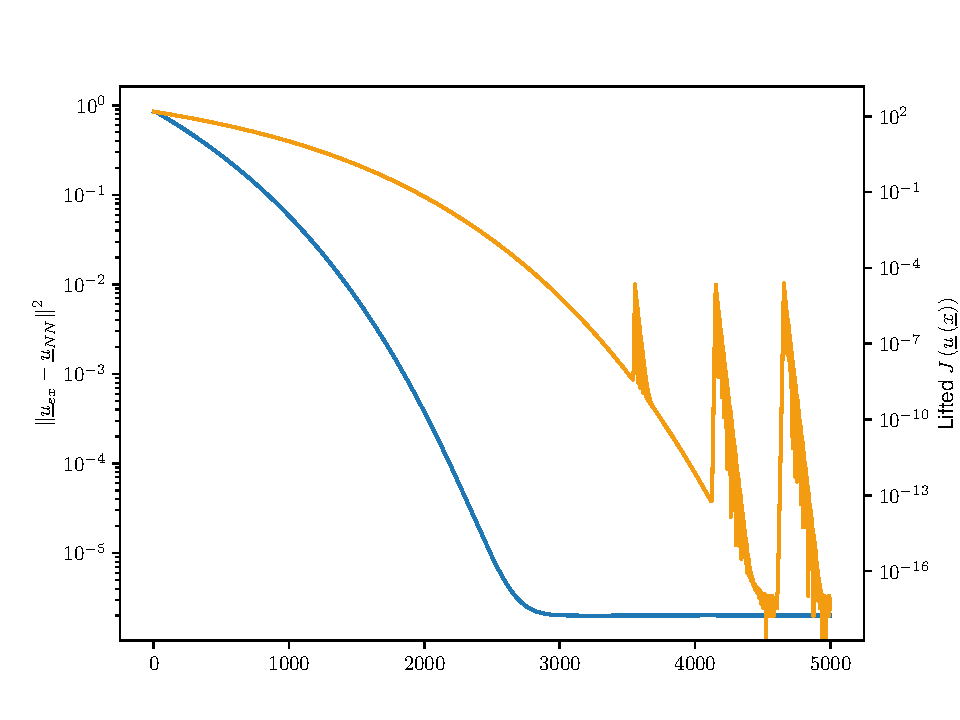
\includegraphics[width=\linewidth]{Figures/Loss_Comaprison_10_Frozen.pdf}
        \caption{Evolution of the loss}
    \end{subfigure}
    \begin{subfigure}{0.3\linewidth}
        \centering
        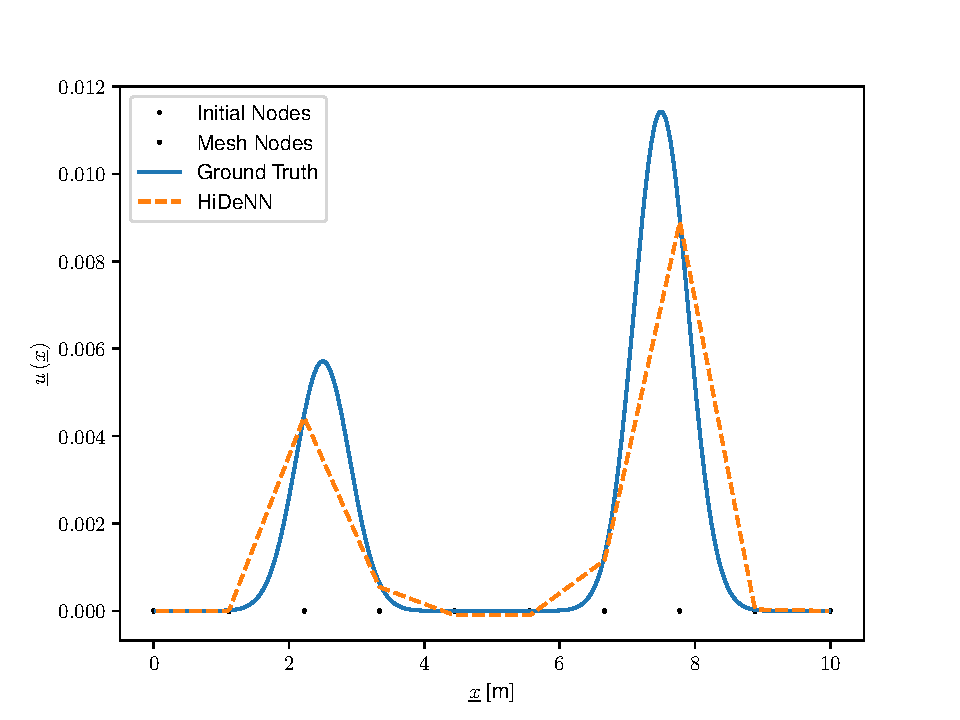
\includegraphics[width=\linewidth]{Figures/Solution_displacement_10_Frozen.pdf}
        \caption{Displacement}
    \end{subfigure}
    \begin{subfigure}{0.3\linewidth}
        \centering
        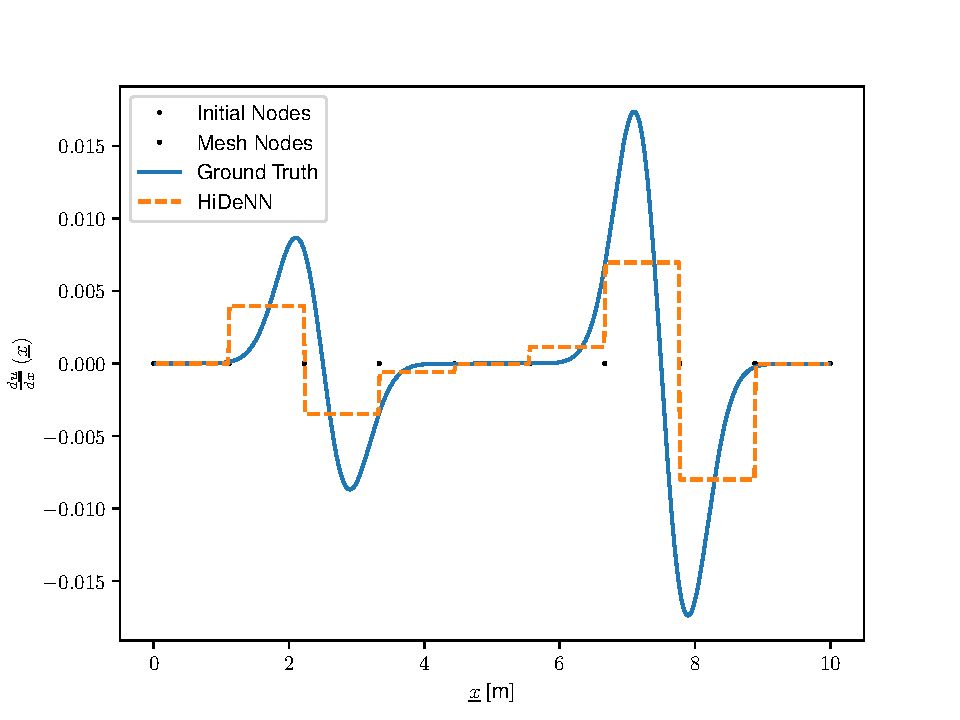
\includegraphics[width=\linewidth]{Figures/Solution_gradients_10_Frozen.pdf}
        \caption{Gradient}
    \end{subfigure}
    \caption{Frozen mesh - $n_p=10$}
    \label{fig:Fixed_Mesh10Float64}
\end{figure}

\begin{figure}
    \begin{subfigure}{0.3\linewidth}
        \centering
        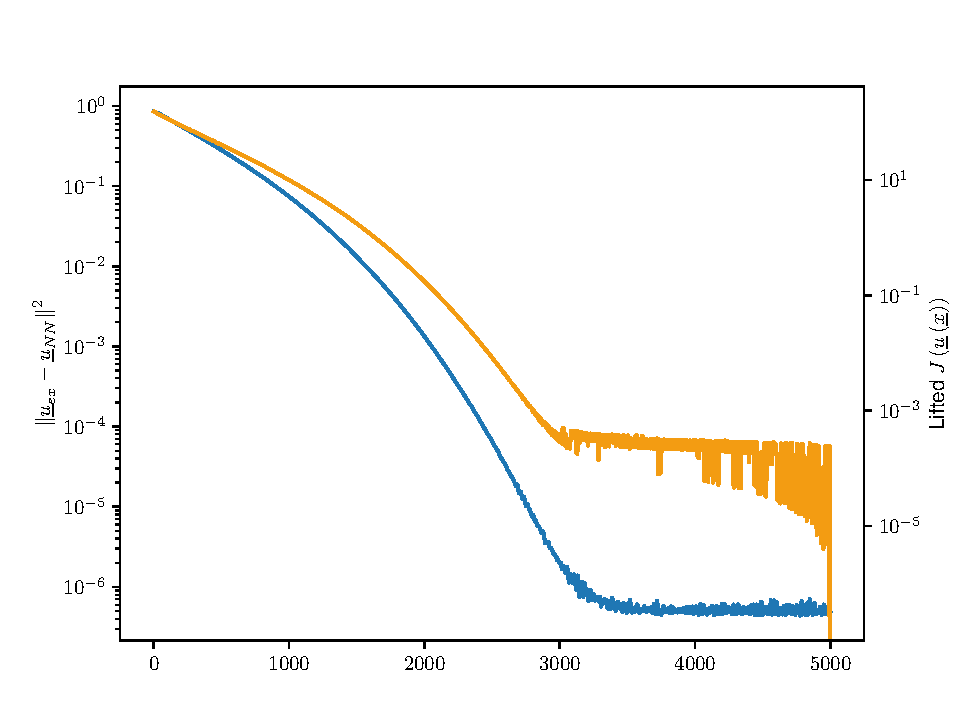
\includegraphics[width=\linewidth]{Figures/Loss_Comaprison_10_Regul.pdf}
        \caption{Evolution of the loss}
    \end{subfigure}
    \begin{subfigure}{0.3\linewidth}
        \centering
        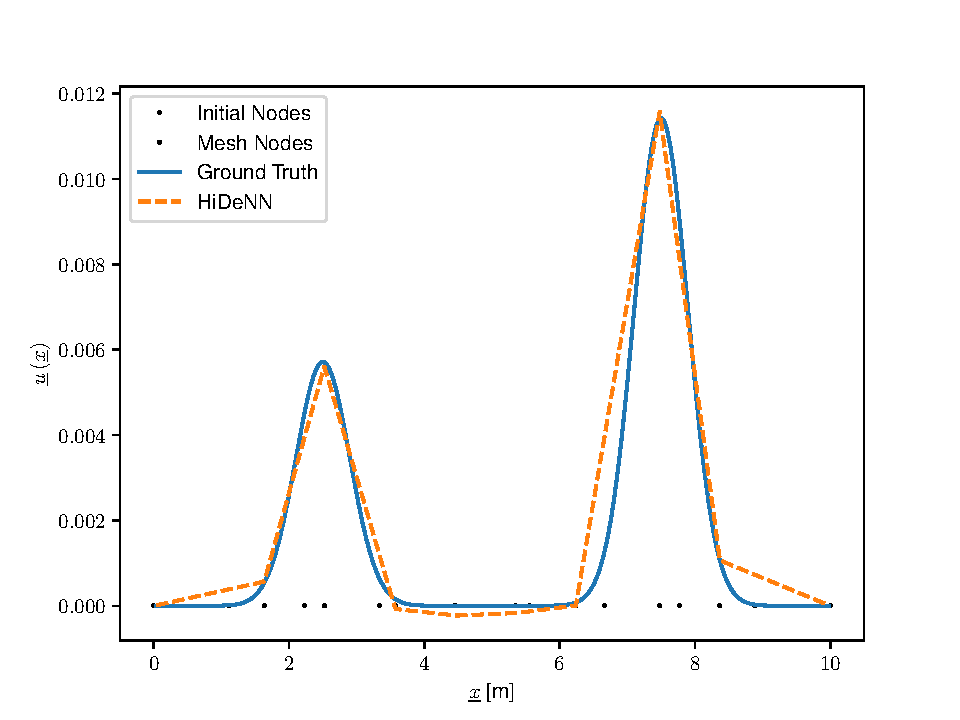
\includegraphics[width=\linewidth]{Figures/Solution_displacement_10_Regul.pdf}
        \caption{Displacement}
    \end{subfigure}
    \begin{subfigure}{0.3\linewidth}
        \centering
        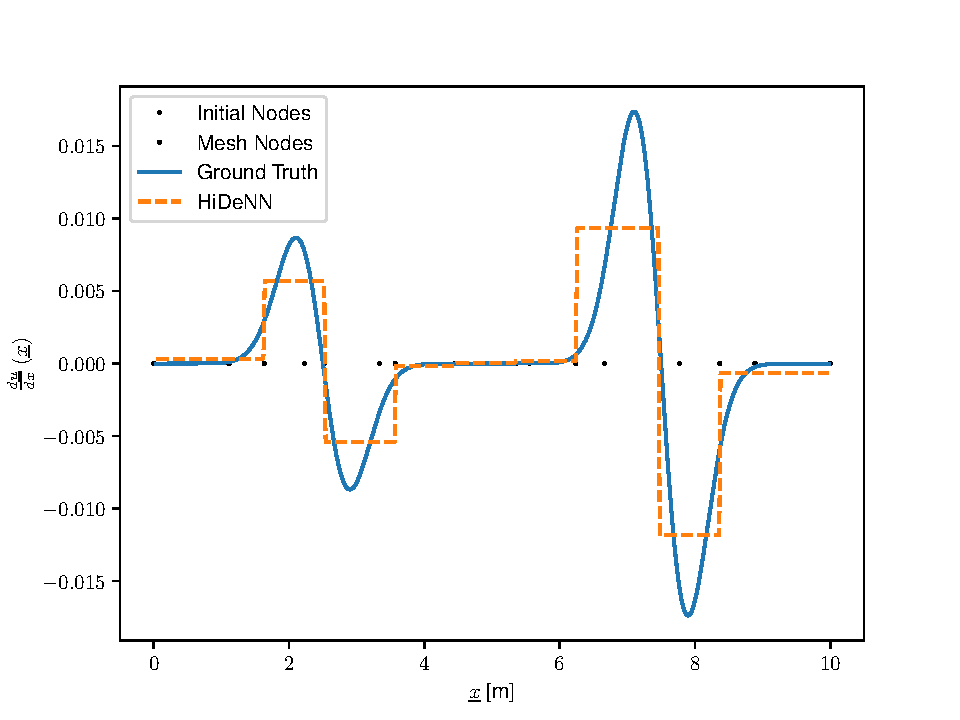
\includegraphics[width=\linewidth]{Figures/Solution_gradients_10_Regul.pdf}
        \caption{Gradient}
    \end{subfigure}
    \caption{Free mesh - $n_p=10$}
    \label{fig:Free_Mesh10Float64}
\end{figure}